\documentclass{article}
\usepackage{amsmath}
\usepackage{pgfplots}
\pgfplotsset{compat=1.16}

\begin{document}

\begin{figure}[h]
    \centering
    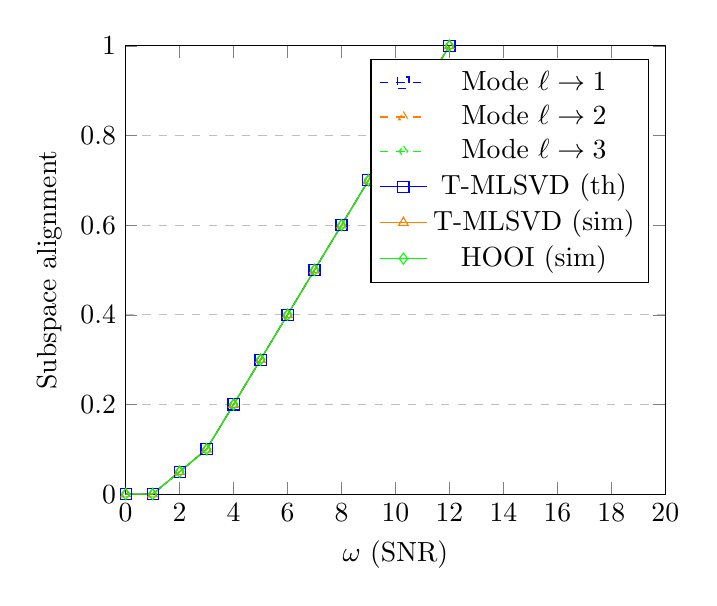
\begin{tikzpicture}
        \begin{axis}[
            xlabel={$\omega$ (SNR)},
            ylabel={Subspace alignment},
            xmin=0, xmax=20,
            ymin=0, ymax=1,
            xtick={0,2,...,20},
            ytick={0,0.2,...,1},
            legend pos=north east,
            ymajorgrids=true,
            grid style=dashed,
        ]
        
        % Mode 1
        \addplot[
            color=blue,
            mark=square,
            dashed,
            error bars/.cd,
            y dir=both,
            y explicit,
            error bar style={line width=0.5pt},
        ]
        coordinates {
            (0,0) (1,0) (2,0.05) (3,0.1) (4,0.2) (5,0.3) (6,0.4) (7,0.5) (8,0.6) (9,0.7) (10,0.8) (11,0.9) (12,1)
        };
        \addlegendentry{Mode $\ell \rightarrow 1$}
        
        % Mode 2
        \addplot[
            color=orange,
            mark=triangle,
            dashed,
            error bars/.cd,
            y dir=both,
            y explicit,
            error bar style={line width=0.5pt},
        ]
        coordinates {
            (0,0) (1,0) (2,0.05) (3,0.1) (4,0.2) (5,0.3) (6,0.4) (7,0.5) (8,0.6) (9,0.7) (10,0.8) (11,0.9) (12,1)
        };
        \addlegendentry{Mode $\ell \rightarrow 2$}
        
        % Mode 3
        \addplot[
            color=green,
            mark=diamond,
            dashed,
            error bars/.cd,
            y dir=both,
            y explicit,
            error bar style={line width=0.5pt},
        ]
        coordinates {
            (0,0) (1,0) (2,0.05) (3,0.1) (4,0.2) (5,0.3) (6,0.4) (7,0.5) (8,0.6) (9,0.7) (10,0.8) (11,0.9) (12,1)
        };
        \addlegendentry{Mode $\ell \rightarrow 3$}
        
        % T-MLSVD (th)
        \addplot[
            color=blue,
            mark=square,
            solid,
            error bars/.cd,
            y dir=both,
            y explicit,
            error bar style={line width=0.5pt},
        ]
        coordinates {
            (0,0) (1,0) (2,0.05) (3,0.1) (4,0.2) (5,0.3) (6,0.4) (7,0.5) (8,0.6) (9,0.7) (10,0.8) (11,0.9) (12,1)
        };
        \addlegendentry{T-MLSVD (th)}
        
        % T-MLSVD (sim)
        \addplot[
            color=orange,
            mark=triangle,
            solid,
            error bars/.cd,
            y dir=both,
            y explicit,
            error bar style={line width=0.5pt},
        ]
        coordinates {
            (0,0) (1,0) (2,0.05) (3,0.1) (4,0.2) (5,0.3) (6,0.4) (7,0.5) (8,0.6) (9,0.7) (10,0.8) (11,0.9) (12,1)
        };
        \addlegendentry{T-MLSVD (sim)}
        
        % HOOI (sim)
        \addplot[
            color=green,
            mark=diamond,
            solid,
            error bars/.cd,
            y dir=both,
            y explicit,
            error bar style={line width=0.5pt},
        ]
        coordinates {
            (0,0) (1,0) (2,0.05) (3,0.1) (4,0.2) (5,0.3) (6,0.4) (7,0.5) (8,0.6) (9,0.7) (10,0.8) (11,0.9) (12,1)
        };
        \addlegendentry{HOOI (sim)}
        
        \end{axis}
    \end{tikzpicture}
    
    \caption{Alignments between singular subspaces (see Section \ref{sec:analysis:reconstruction}) of the observation ${\bm{\mathscr{T}}} = \sqrt{\omega}{\bm{\mathscr{P}}}_\circ + \frac{1}{\sqrt{N}}{\bm{\mathscr{N}}}$ and of the signal ${\bm{\mathscr{P}}}_\circ$, with $\lVert{\bm{\mathscr{P}}}_\circ \rVert_{\mathrm{F}}^2 = \frac{\sqrt{n_1 n_2 n_3}}{N}$, as a function of the signal-to-noise ratio $\omega$. Theoretical alignments (Theorem \ref{thm:spike}) achieved with truncated MLSVD are compared with simulations and those achieved with the HOOI algorithm. Empirical results are averaged over $10$ trials, with error bars representing standard deviation. \textbf{Experimental setting:} $d = 3$, $(n_1, n_2, n_3) = (100, 200, 300)$, $N = n_1 + n_2 + n_3$ and $(r_1, r_2, r_3) = (3, 4, 5)$.}
    \label{fig:subspace_alignment}
\end{figure}

\end{document}